\documentclass[12pt]{article}
\usepackage{fullpage}
\usepackage{graphicx}

\usepackage{Sweave}
\begin{document}
\Sconcordance{concordance:PS2.tex:PS2.Rnw:%
1 4 1 1 0 10 1 1 3 2 0 1 1 1 2 2 1 14 0 1 2 3 1 1 2 1 0 1 1 33 0 1 3 2 %
1 1 2 2 1 1 2 1 0 1 1 34 0 1 3 7 1 1 2 1 0 1 2 1 1 30 0 2 2 1 0 1 1 58 %
0 1 2 7 1 1 2 1 0 5 1 6 0 1 4 2 0 1 6 4 0 1 6 4 0 1 2 3 0 1 2 6 1}


\pagestyle{empty}

\begin{center}
{\Large \textbf{POLS 500c: Problem Set \# 3}}
\end{center}

The dataset \texttt{Obama.dta} is a subset of the 2008 American National Election Survey.  We will use it to examine attitudes toward Barack Obama, using the feeling thermometer \texttt{obama}.

\begin{Schunk}
\begin{Sinput}
> # Setup
> require(foreign)
> obama <- read.dta("Obama.dta")
> var.labels <- attr(obama,"var.labels")
> data.key <- data.frame(var.name=names(obama),var.labels)
> data.key
\end{Sinput}
\begin{Soutput}
  var.name                      var.labels
1    obama       Obama feeling thermometer
2      age                    Years of age
3   income         Household income, $000s
4     educ              Years of education
5   female                          Female
6    black      R self-identifies as black
7      dem   R self-identifies as Democrat
8      rep R self-identifies as Republican
\end{Soutput}
\end{Schunk}

\begin{enumerate}
\item Suppose we hypothesize that a respondent's income affects her or his attitudes toward Obama, that those with higher incomes will express cooler feelings toward him.  Controlling for age, education, gender, race, and partisanship, is this hypothesis supported?  How do you know?

\begin{Schunk}
\begin{Sinput}
> m1<-lm(obama ~ income + age + educ + female + black + dem + rep,data=obama)
> summary(m1)
\end{Sinput}
\begin{Soutput}
Call:
lm(formula = obama ~ income + age + educ + female + black + dem + 
    rep, data = obama)

Residuals:
    Min      1Q  Median      3Q     Max 
-75.815 -11.761   3.395  12.594  66.320 

Coefficients:
             Estimate Std. Error t value Pr(>|t|)    
(Intercept)  60.20277    3.24800  18.535  < 2e-16 ***
income       -0.03332    0.01043  -3.193  0.00143 ** 
age          -0.03495    0.03013  -1.160  0.24629    
educ          0.04891    0.21070   0.232  0.81647    
female        4.48527    0.99574   4.504 7.07e-06 ***
black        16.76626    1.22609  13.675  < 2e-16 ***
dem          13.76778    1.14550  12.019  < 2e-16 ***
rep         -16.71796    1.40899 -11.865  < 2e-16 ***
---
Signif. codes:  0 '***' 0.001 '**' 0.01 '*' 0.05 '.' 0.1 ' ' 1

Residual standard error: 21.03 on 1850 degrees of freedom
  (465 observations deleted due to missingness)
Multiple R-squared:  0.3779,	Adjusted R-squared:  0.3756 
F-statistic: 160.6 on 7 and 1850 DF,  p-value: < 2.2e-16
\end{Soutput}
\begin{Sinput}
> 
\end{Sinput}
\end{Schunk}
In order to test the hypothesis we use linear regression to see whether there is any relationship between the income of a respondent and his or her attitude toward Obama.  The Obama feeling theromometer (variable:obama) is set as the dependent variable . 
As we can see "income=-0.03332" from these results, the income of a respondent has a statistically significant effect on his or her atttitude towards Obama. With an increment of one thousands dollars in personal income, feeling towards Obama decreases by 0.033.  Thus the result supports our hypothesis that those with higher incomes will express cooler feelings toward him.


\item Suppose we think Democrats' feelings toward Obama will be less influenced by their incomes than others' feelings are.  Is there support for this conditional hypothesis?  How do you know?\\

\begin{Schunk}
\begin{Sinput}
> m2<-lm(obama ~ income + dem + dem:income + rep + age + educ + female + black, data=obama)
> summary(m2)
\end{Sinput}
\begin{Soutput}
Call:
lm(formula = obama ~ income + dem + dem:income + rep + age + 
    educ + female + black, data = obama)

Residuals:
   Min     1Q Median     3Q    Max 
-76.67 -11.64   3.05  12.73  69.79 

Coefficients:
              Estimate Std. Error t value Pr(>|t|)    
(Intercept)  61.666783   3.271568  18.849  < 2e-16 ***
income       -0.053484   0.012147  -4.403 1.13e-05 ***
dem          10.504224   1.527455   6.877 8.34e-12 ***
rep         -16.009862   1.422543 -11.254  < 2e-16 ***
age          -0.030398   0.030092  -1.010  0.31255    
educ         -0.004112   0.210809  -0.020  0.98444    
female        4.433373   0.993360   4.463 8.57e-06 ***
black        17.070766   1.226655  13.917  < 2e-16 ***
income:dem    0.067813   0.021063   3.219  0.00131 ** 
---
Signif. codes:  0 '***' 0.001 '**' 0.01 '*' 0.05 '.' 0.1 ' ' 1

Residual standard error: 20.97 on 1849 degrees of freedom
  (465 observations deleted due to missingness)
Multiple R-squared:  0.3814,	Adjusted R-squared:  0.3787 
F-statistic: 142.5 on 8 and 1849 DF,  p-value: < 2.2e-16
\end{Soutput}
\begin{Sinput}
> 
\end{Sinput}
\end{Schunk}
In order to test the conditional hypothesis and see how being a Democrat influences the effect of income on feelings toward Obama, we add an interaction term of "dem*income" as an additional independent variable into the linear model.  
  
As we can see "income=-0.053484" and "income:dem=.067813".  To calculate the effect of income on Democrats we simply add the coefficient for the interaction term to the coefficient for the constitutive term: -.053484 + .067813 = .014329.  The effect of income when dem = 0 is the coefficient for income, -.053484.  Not only is there a much smaller effect of income for Democrats on feelings toward Obama, the effect is in the opposite, positive direction.

These results support our hypothesis that Democrats are less influence by their incomes than others' feelings are when considering feelings toward Obama.

\item Does income have a statistically significant effect on the feelings toward Obama of those who aren't Democrats?  On the feelings of Democrats?  Report the estimated effect and $p$-value for each.\\

\begin{Schunk}
\begin{Sinput}
> nondem<-ifelse(obama$dem==0,1,0)
> m3<-lm(obama ~ income + nondem:income + age + educ + female + black + nondem,data=obama)
> summary(m3)
\end{Sinput}
\begin{Soutput}
Call:
lm(formula = obama ~ income + nondem:income + age + educ + female + 
    black + nondem, data = obama)

Residuals:
    Min      1Q  Median      3Q     Max 
-77.075 -10.065   1.828  12.986  66.655 

Coefficients:
               Estimate Std. Error t value Pr(>|t|)    
(Intercept)    75.67523    3.53907  21.383  < 2e-16 ***
income          0.01925    0.01869   1.030   0.3032    
age            -0.06819    0.03090  -2.207   0.0275 *  
educ           -0.17733    0.21727  -0.816   0.4145    
female          4.13791    1.02618   4.032 5.75e-05 ***
black          18.35369    1.26215  14.542  < 2e-16 ***
nondem        -13.51130    1.55414  -8.694  < 2e-16 ***
income:nondem  -0.10446    0.02151  -4.858 1.29e-06 ***
---
Signif. codes:  0 '***' 0.001 '**' 0.01 '*' 0.05 '.' 0.1 ' ' 1

Residual standard error: 21.67 on 1850 degrees of freedom
  (465 observations deleted due to missingness)
Multiple R-squared:  0.339,	Adjusted R-squared:  0.3365 
F-statistic: 135.5 on 7 and 1850 DF,  p-value: < 2.2e-16
\end{Soutput}
\end{Schunk}

\begin{Schunk}
\begin{Sinput}
> library(stargazer)
> stargazer(m1,m2,m3,title="Linear regression Results",dep.var.labels="Attitude towards Barack Obama", align=TRUE, omit.stat=c("adj.rsq","f","ser"),label="T:res")
\end{Sinput}
% Table created by stargazer v.4.5.3 by Marek Hlavac, Harvard University. E-mail: hlavac at fas.harvard.edu
% Date and time: Mon, Mar 03, 2014 - 10:56:57 AM
% Requires LaTeX packages: dcolumn 
\begin{table}[!htbp] \centering 
  \caption{Linear regression Results} 
  \label{T:res} 
\begin{tabular}{@{\extracolsep{5pt}}lD{.}{.}{-3} D{.}{.}{-3} D{.}{.}{-3} } 
\\[-1.8ex]\hline 
\hline \\[-1.8ex] 
 & \multicolumn{3}{c}{\textit{Dependent variable:}} \\ 
\cline{2-4} 
\\[-1.8ex] & \multicolumn{3}{c}{Attitude towards Barack Obama} \\ 
\\[-1.8ex] & \multicolumn{1}{c}{(1)} & \multicolumn{1}{c}{(2)} & \multicolumn{1}{c}{(3)}\\ 
\hline \\[-1.8ex] 
 income & -0.033^{***} & -0.053^{***} & 0.019 \\ 
  & (0.010) & (0.012) & (0.019) \\ 
  & & & \\ 
 age & -0.035 & -0.030 & -0.068^{**} \\ 
  & (0.030) & (0.030) & (0.031) \\ 
  & & & \\ 
 educ & 0.049 & -0.004 & -0.177 \\ 
  & (0.211) & (0.211) & (0.217) \\ 
  & & & \\ 
 female & 4.485^{***} & 4.433^{***} & 4.138^{***} \\ 
  & (0.996) & (0.993) & (1.026) \\ 
  & & & \\ 
 black & 16.766^{***} & 17.071^{***} & 18.354^{***} \\ 
  & (1.226) & (1.227) & (1.262) \\ 
  & & & \\ 
 income:dem &  & 0.068^{***} &  \\ 
  &  & (0.021) &  \\ 
  & & & \\ 
 dem & 13.768^{***} & 10.504^{***} &  \\ 
  & (1.145) & (1.527) &  \\ 
  & & & \\ 
 rep & -16.718^{***} & -16.010^{***} &  \\ 
  & (1.409) & (1.423) &  \\ 
  & & & \\ 
 nondem &  &  & -13.511^{***} \\ 
  &  &  & (1.554) \\ 
  & & & \\ 
 income:nondem &  &  & -0.104^{***} \\ 
  &  &  & (0.022) \\ 
  & & & \\ 
 Constant & 60.203^{***} & 61.667^{***} & 75.675^{***} \\ 
  & (3.248) & (3.272) & (3.539) \\ 
  & & & \\ 
\hline \\[-1.8ex] 
Observations & \multicolumn{1}{c}{1,858} & \multicolumn{1}{c}{1,858} & \multicolumn{1}{c}{1,858} \\ 
R$^{2}$ & \multicolumn{1}{c}{0.378} & \multicolumn{1}{c}{0.381} & \multicolumn{1}{c}{0.339} \\ 
\hline 
\hline \\[-1.8ex] 
\textit{Note:}  & \multicolumn{3}{r}{$^{*}$p$<$0.1; $^{**}$p$<$0.05; $^{***}$p$<$0.01} \\ 
\normalsize 
\end{tabular} 
\end{table} \end{Schunk}


From these results we can see income has a statistically significant effect on non-Democrats feeling towards Obama (coefficient:-0.10446). For every thousand dollar increase in income feeling towards Obama decreases by .10446 among non-Democrats, an effect significant at the .05 level.  

Using this coding scheme for partisanship we see our results from Question 2 verified in this model: the coefficient for income (when nondem=0, or for Democratic respondents) is equal to .019, roughly the size of the coefficient estimated earlier.  In addition, this effect is not statistically significant.  That is, income does not influence feelings toward Obama among Democrats in this model.  It does, however, influence non-Democrats.  

\item Suppose we were really more interested in how being a Democrat affects feelings towards Obama.  What effect does income have on this effect?  Graph your answer and insert the graph in your \LaTeX~file.\\

\begin{Schunk}
\begin{Sinput}
> library(arm)
> library(ggplot2)
> set.seed(740)
> n.sims=9999
> m2.sims <- sim(m2, n.sims)
> apply(m2.sims@coef, 2, mean)
\end{Sinput}
\begin{Soutput}
[1]  61.660639647  -0.053385807  10.502757831 -16.002200114  -0.030415168
[6]  -0.005178129   4.442292229  17.076609333   0.068027834
\end{Soutput}
\begin{Sinput}
> display(m2)
\end{Sinput}
\begin{Soutput}
lm(formula = obama ~ income + dem + dem:income + rep + age + 
    educ + female + black, data = obama)
            coef.est coef.se
(Intercept)  61.67     3.27 
income       -0.05     0.01 
dem          10.50     1.53 
rep         -16.01     1.42 
age          -0.03     0.03 
educ          0.00     0.21 
female        4.43     0.99 
black        17.07     1.23 
income:dem    0.07     0.02 
---
n = 1858, k = 9
residual sd = 20.97, R-Squared = 0.38
\end{Soutput}
\begin{Sinput}
> coef.dem <- data.frame(fake_income = seq(min(obama$income, na.rm=T), 
+                                          max(obama$income, na.rm=T), 
+                         length.out=100), coef_dem = NA, ub_dem = NA, lb_dem = NA) 
> for(i in 1:100) {   
+     coef.dem$coef_dem[i] <- mean(m2.sims@coef[,7] + coef.dem$fake_income[i]*m2.sims@coef[,8])
+     coef.dem$ub_dem[i] <- quantile(m2.sims@coef[,7] + coef.dem$fake_income[i]*m2.sims@coef[,8], .975)
+     coef.dem$lb_dem[i] <- quantile(m2.sims@coef[,7] + coef.dem$fake_income[i]*m2.sims@coef[,8], .025)    
+ } 
> dem.coef.plot <- ggplot(coef.dem, aes(x = fake_income, y = coef_dem)) + 
+     geom_line() + geom_ribbon(aes(ymin=lb_dem, ymax=ub_dem), alpha=.5) +
+     xlab("Household income, $000s") + ylab("Coefficient of Democrats") +
+     scale_x_continuous(limits=c(0,80)) + 
+     scale_y_continuous(limits=c(0,2000))
> dem.coef.plot
\end{Sinput}
\end{Schunk}

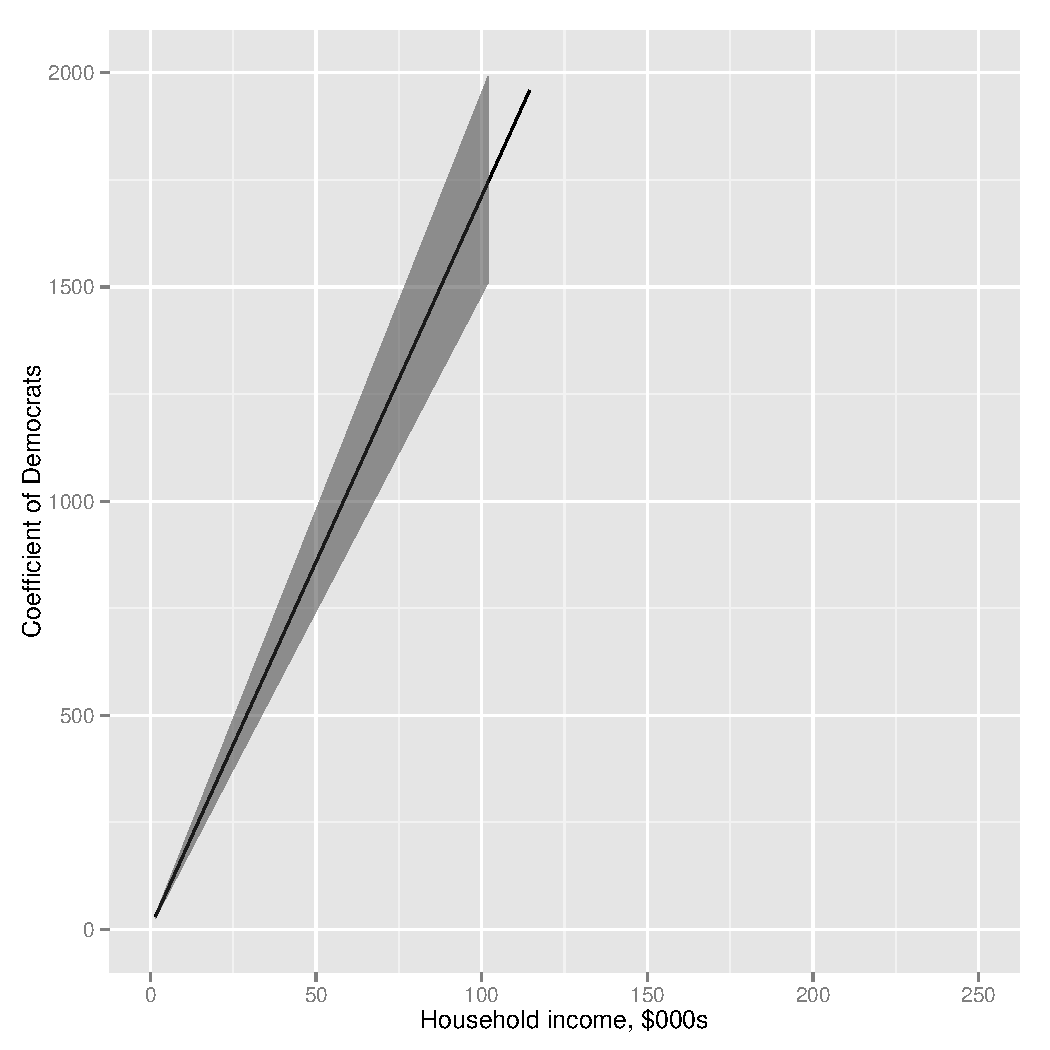
\includegraphics{Rplots.pdf}

From the simulated results we graphed income against the coefficient for the dem variable, including 95\% confidence intervals.  There appears to be a positive effect of income for Democrats on feelings toward Obama.

\end{enumerate}
\end{document}
